%==============================================================
%  Figura A.1 - Valutazione del rischio per i dispositivi di
%  protezione del bordo di chiusura di finestre, porte e cancelli
%  motorizzati (Allegato A, Esempio 1)
%  Adattamento in italiano della Figura A.1 dell'IFA Report 2/2017
%
%  Le coordinate sono ricavate dal disegno di partenza (1 cm = 70 px,
%  origine nell'angolo in alto a sinistra della cornice). Il disegno
%  del cancello e' riprodotto con i segmenti verticali e orizzontali
%  misurati sull'originale (spessore e tono di grigio compresi); il
%  montante punteggiato, il bordo di chiusura nero, la freccia e le
%  ruote sono disegnati a parte. Nessun cambio di corpo del font.
%==============================================================
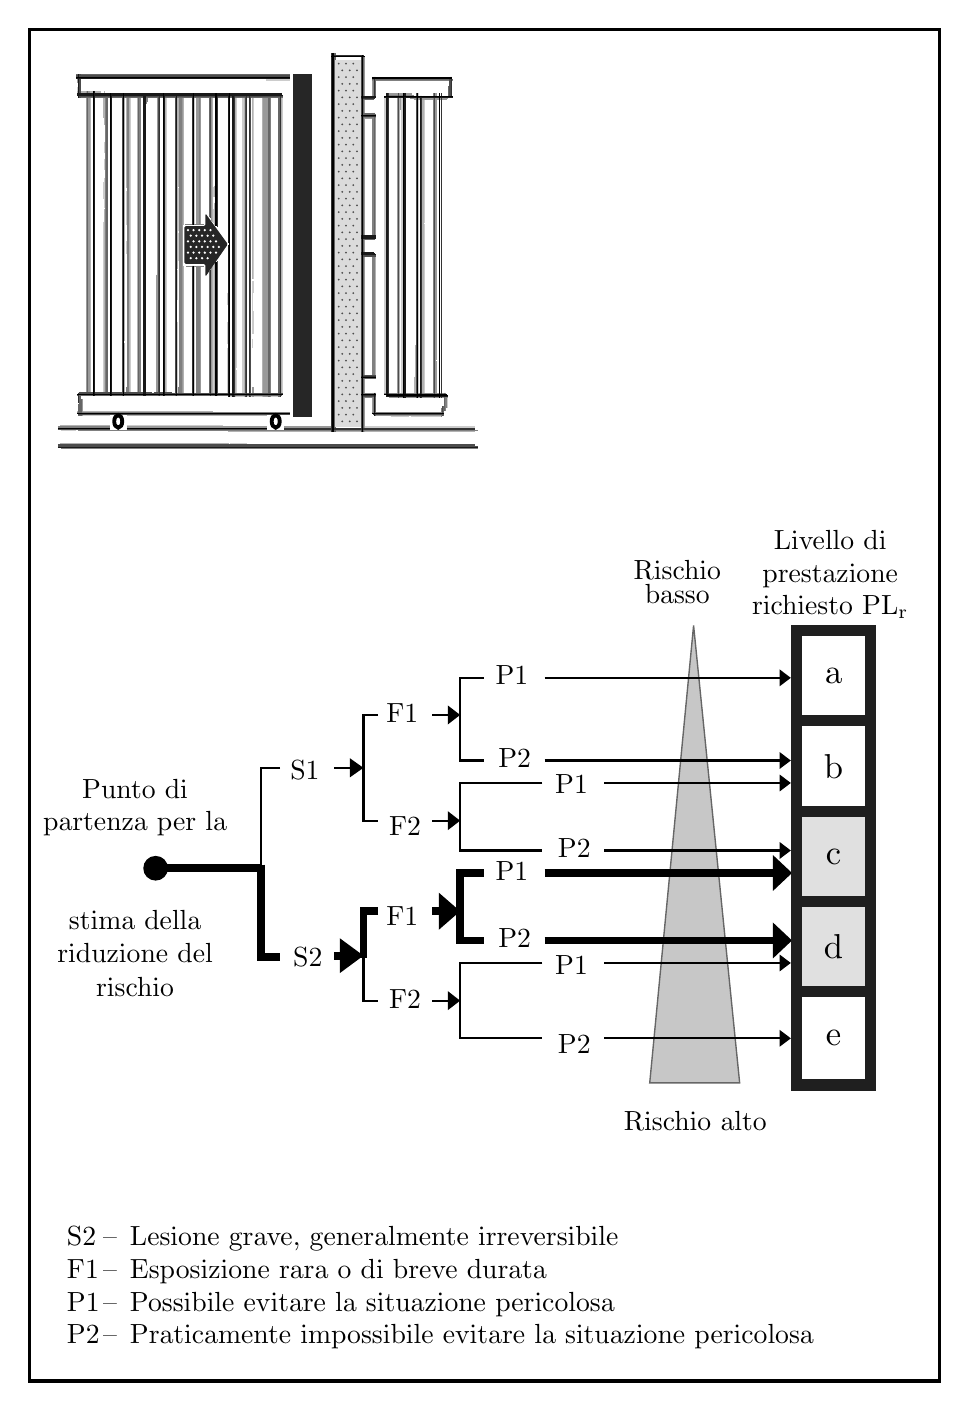
\begin{tikzpicture}[
  font=\normalsize,
  sottile/.style={draw=black, line width=0.8pt},
  spesso/.style={draw=black, line width=2.8pt},
  etichetta/.style={inner sep=0pt},
  lettera/.style={inner sep=0pt, scale=1.25}
]

%--------------------------------------------------------------
% Cornice
%--------------------------------------------------------------
\draw[draw=black, line width=1.2pt] (0.000,-0.000) rectangle (11.557,-17.164);

%--------------------------------------------------------------
% Cancello scorrevole motorizzato: segmenti verticali e orizzontali
%--------------------------------------------------------------
\draw[line width=0.406pt, draw=black!20] (0.614,-0.729) -- (0.614,-0.843) (0.943,-1.943) -- (0.943,-2.157) (0.943,-2.443) -- (0.943,-4.657) (0.957,-1.429) -- (0.957,-1.571) (0.957,-1.643) -- (0.957,-1.786) (0.957,-1.886) -- (0.957,-2.271) (1.229,-2.057) -- (1.229,-2.486) (1.229,-2.686) -- (1.229,-2.857) (1.286,-0.814) -- (1.286,-4.657) (1.743,-0.814) -- (1.743,-4.657) (1.886,-3.057) -- (1.886,-3.443) (1.886,-3.714) -- (1.886,-4.657) (1.900,-2.014) -- (1.900,-2.557) (1.900,-2.586) -- (1.900,-2.943) (2.100,-0.814) -- (2.100,-2.486) (2.100,-3.000) -- (2.100,-4.657) (2.343,-2.000) -- (2.343,-2.129) (2.343,-2.286) -- (2.343,-2.457) (2.343,-3.000) -- (2.343,-4.657) (2.514,-3.343) -- (2.514,-3.500) (2.514,-3.714) -- (2.514,-4.000) (2.514,-4.043) -- (2.514,-4.657) (2.629,-0.814) -- (2.629,-4.300) (2.629,-4.329) -- (2.629,-4.671) (2.714,-0.814) -- (2.714,-4.671) (2.829,-3.200) -- (2.829,-3.871) (2.829,-3.929) -- (2.829,-4.043) (2.843,-0.814) -- (2.843,-3.171) (2.843,-3.200) -- (2.843,-3.343) (2.843,-3.571) -- (2.843,-3.871) (3.214,-0.829) -- (3.214,-4.643) (4.514,-0.843) -- (4.514,-4.643) (4.529,-0.843) -- (4.529,-4.643) (4.729,-0.814) -- (4.729,-4.686) (4.743,-0.814) -- (4.743,-4.686) (4.943,-0.814) -- (4.943,-4.686) (5.014,-0.843) -- (5.014,-2.457) (5.014,-2.471) -- (5.014,-4.686) (5.314,-4.643) -- (5.314,-4.814) (3.007,-0.636) -- (3.307,-0.636) (3.007,-0.650) -- (3.307,-0.650) (2.521,-4.664) -- (3.193,-4.664) (0.621,-4.907) -- (1.021,-4.907) (4.593,-4.921) -- (4.821,-4.921) (4.850,-4.921) -- (5.236,-4.921) (1.236,-5.036) -- (2.464,-5.036) (4.207,-5.050) -- (5.664,-5.050) (0.407,-5.093) -- (0.593,-5.093) (2.550,-5.264) -- (2.764,-5.264);
\draw[line width=0.406pt, draw=black!30] (0.771,-0.786) -- (0.771,-4.657) (0.943,-0.814) -- (0.943,-1.129) (0.957,-0.786) -- (0.957,-1.214) (0.957,-2.286) -- (0.957,-4.657) (1.214,-0.814) -- (1.214,-3.957) (1.214,-3.986) -- (1.214,-4.657) (1.229,-0.814) -- (1.229,-2.014) (1.271,-0.814) -- (1.271,-4.657) (1.371,-0.814) -- (1.371,-4.657) (1.729,-0.814) -- (1.729,-4.657) (1.886,-0.814) -- (1.886,-3.043) (1.900,-0.814) -- (1.900,-2.000) (1.957,-0.814) -- (1.957,-2.486) (1.957,-3.000) -- (1.957,-4.657) (2.329,-0.814) -- (2.329,-2.443) (2.329,-3.014) -- (2.329,-4.657) (2.357,-1.986) -- (2.357,-2.129) (2.357,-2.200) -- (2.357,-2.486) (2.357,-2.971) -- (2.357,-4.657) (2.614,-0.814) -- (2.614,-4.671) (2.729,-0.814) -- (2.729,-4.671) (2.829,-0.814) -- (2.829,-3.171) (2.957,-0.814) -- (2.957,-4.671) (3.200,-0.814) -- (3.200,-4.657) (4.400,-2.857) -- (4.400,-4.443) (4.700,-0.814) -- (4.700,-4.686) (4.886,-4.414) -- (4.886,-4.686) (4.900,-4.014) -- (4.900,-4.686) (5.000,-0.843) -- (5.000,-4.686) (0.607,-0.793) -- (0.907,-0.793) (0.607,-0.807) -- (0.907,-0.807) (0.607,-4.850) -- (2.336,-4.850) (1.236,-4.907) -- (3.021,-4.907) (0.393,-5.036) -- (1.021,-5.036) (2.521,-5.107) -- (5.664,-5.107) (0.393,-5.264) -- (2.536,-5.264);
\draw[line width=0.406pt, draw=black!40] (0.614,-0.571) -- (0.614,-0.686) (0.671,-4.700) -- (0.671,-4.914) (0.729,-0.786) -- (0.729,-4.657) (0.757,-0.786) -- (0.757,-4.657) (1.614,-3.114) -- (1.614,-4.657) (1.629,-0.814) -- (1.629,-4.657) (1.943,-0.814) -- (1.943,-4.657) (2.129,-0.814) -- (2.129,-2.486) (2.143,-0.814) -- (2.143,-2.486) (2.171,-0.814) -- (2.171,-2.486) (2.171,-3.000) -- (2.171,-4.657) (2.314,-0.814) -- (2.314,-2.429) (2.314,-3.029) -- (2.314,-4.657) (2.829,-4.543) -- (2.829,-4.671) (2.843,-4.543) -- (2.843,-4.671) (2.971,-0.814) -- (2.971,-4.671) (2.986,-0.814) -- (2.986,-4.671) (3.000,-0.814) -- (3.000,-4.671) (3.014,-0.814) -- (3.014,-4.671) (3.029,-0.814) -- (3.029,-4.671) (4.257,-0.343) -- (4.257,-5.114) (4.357,-0.600) -- (4.357,-0.900) (4.357,-4.614) -- (4.357,-4.886) (4.400,-1.071) -- (4.400,-2.657) (4.671,-0.814) -- (4.671,-4.686) (4.714,-0.814) -- (4.714,-1.029) (5.157,-0.814) -- (5.157,-4.686) (5.171,-0.814) -- (5.171,-4.200) (5.171,-4.214) -- (5.171,-4.686) (4.536,-0.821) -- (4.864,-0.821) (4.836,-0.879) -- (5.321,-0.879) (4.879,-0.893) -- (5.307,-0.893) (4.207,-1.136) -- (4.407,-1.136) (4.564,-4.679) -- (5.321,-4.679) (4.379,-4.907) -- (5.264,-4.907) (1.236,-5.050) -- (3.021,-5.050) (3.236,-5.050) -- (3.893,-5.050);
\draw[line width=0.406pt, draw=black!50] (0.971,-0.814) -- (0.971,-4.657) (1.229,-4.543) -- (1.229,-4.657) (1.243,-0.814) -- (1.243,-4.657) (1.257,-0.814) -- (1.257,-4.657) (1.400,-0.814) -- (1.400,-4.657) (1.414,-0.814) -- (1.414,-4.657) (1.486,-0.814) -- (1.486,-0.943) (1.500,-0.814) -- (1.500,-0.929) (1.900,-4.543) -- (1.900,-4.657) (1.914,-0.814) -- (1.914,-4.657) (1.929,-0.814) -- (1.929,-4.657) (2.129,-3.000) -- (2.129,-4.657) (2.143,-3.000) -- (2.143,-4.657) (2.157,-0.814) -- (2.157,-2.486) (2.157,-3.000) -- (2.157,-4.657) (3.057,-0.814) -- (3.057,-4.671) (4.357,-1.057) -- (4.357,-2.671) (4.357,-2.829) -- (4.357,-4.443) (4.371,-0.600) -- (4.371,-0.900) (4.371,-1.057) -- (4.371,-2.671) (4.371,-2.829) -- (4.371,-4.443) (4.371,-4.614) -- (4.371,-4.900) (4.386,-2.843) -- (4.386,-4.443) (5.129,-0.814) -- (5.129,-4.686) (5.229,-4.814) -- (5.229,-4.929) (5.286,-4.614) -- (5.286,-4.843) (5.300,-4.629) -- (5.300,-4.814) (4.350,-0.650) -- (5.379,-0.650) (4.536,-0.836) -- (4.879,-0.836) (4.207,-1.121) -- (4.407,-1.121) (1.979,-2.479) -- (2.221,-2.479) (1.993,-3.007) -- (2.221,-3.007) (4.207,-4.621) -- (4.407,-4.621) (4.507,-4.621) -- (5.293,-4.621) (4.207,-4.679) -- (4.407,-4.679) (0.607,-4.864) -- (3.307,-4.864) (4.350,-4.864) -- (5.264,-4.864) (0.364,-5.050) -- (1.021,-5.050) (0.621,-5.093) -- (5.693,-5.093) (0.407,-5.321) -- (5.693,-5.321);
\draw[line width=0.406pt, draw=black!60] (0.629,-4.757) -- (0.629,-4.914) (0.643,-4.600) -- (0.643,-4.914) (0.657,-4.700) -- (0.657,-4.914) (0.743,-0.786) -- (0.743,-4.657) (0.986,-0.814) -- (0.986,-4.657) (1.386,-0.814) -- (1.386,-4.657) (2.286,-0.814) -- (2.286,-2.386) (2.286,-3.071) -- (2.286,-4.657) (3.043,-0.814) -- (3.043,-4.671) (3.171,-0.814) -- (3.171,-4.671) (3.871,-0.300) -- (3.871,-5.114) (3.886,-0.300) -- (3.886,-5.114) (4.243,-0.329) -- (4.243,-5.114) (4.386,-1.057) -- (4.386,-2.671) (4.400,-0.600) -- (4.400,-0.871) (4.400,-4.614) -- (4.400,-4.914) (5.257,-4.786) -- (5.257,-4.914) (5.271,-4.614) -- (5.271,-4.843) (5.329,-0.714) -- (5.329,-0.871) (0.593,-0.579) -- (3.307,-0.579) (4.350,-0.636) -- (5.379,-0.636) (0.621,-0.864) -- (3.221,-0.864) (4.207,-0.893) -- (4.379,-0.893) (4.207,-1.064) -- (4.393,-1.064) (4.207,-1.079) -- (4.407,-1.079) (4.207,-2.664) -- (4.393,-2.664) (4.207,-4.436) -- (4.407,-4.436) (0.607,-4.650) -- (3.207,-4.650);
\draw[line width=0.406pt, draw=black!70] (0.643,-0.571) -- (0.643,-0.871) (1.186,-0.814) -- (1.186,-4.657) (1.643,-0.814) -- (1.643,-4.657) (1.857,-0.814) -- (1.857,-4.657) (2.300,-0.814) -- (2.300,-2.400) (2.386,-2.943) -- (2.386,-4.657) (2.743,-0.814) -- (2.743,-4.671) (2.814,-0.814) -- (2.814,-4.671) (4.214,-0.329) -- (4.214,-5.114) (4.686,-0.814) -- (4.686,-4.686) (4.914,-0.814) -- (4.914,-4.686) (5.143,-0.814) -- (5.143,-4.686) (5.243,-4.786) -- (5.243,-4.914) (5.343,-0.600) -- (5.343,-0.871) (0.593,-0.593) -- (3.307,-0.593) (0.621,-0.850) -- (3.221,-0.850) (4.207,-2.879) -- (4.407,-2.879) (4.207,-4.393) -- (4.407,-4.393) (0.636,-4.607) -- (1.564,-4.607) (1.579,-4.607) -- (1.807,-4.607) (0.621,-4.621) -- (3.221,-4.621) (4.207,-4.664) -- (4.407,-4.664) (0.621,-4.893) -- (3.307,-4.893) (4.364,-4.893) -- (5.264,-4.893) (0.364,-5.079) -- (1.021,-5.079) (1.236,-5.079) -- (3.021,-5.079) (0.364,-5.279) -- (5.664,-5.279) (0.364,-5.293) -- (5.693,-5.293);
\draw[line width=0.406pt, draw=black!80] (0.629,-4.614) -- (0.629,-4.743) (1.657,-0.814) -- (1.657,-4.657) (2.071,-0.814) -- (2.071,-2.486) (2.071,-3.000) -- (2.071,-4.657) (2.300,-3.057) -- (2.300,-4.657) (2.386,-0.814) -- (2.386,-2.514) (2.600,-0.814) -- (2.600,-4.671) (2.757,-0.814) -- (2.757,-4.671) (2.800,-0.814) -- (2.800,-4.671) (3.186,-0.814) -- (3.186,-4.671) (3.843,-0.300) -- (3.843,-5.114) (4.386,-0.600) -- (4.386,-0.886) (4.557,-0.814) -- (4.557,-4.671) (4.986,-0.843) -- (4.986,-4.686) (5.229,-0.814) -- (5.229,-4.686) (5.357,-0.600) -- (5.357,-0.871) (3.836,-0.336) -- (4.250,-0.336) (4.207,-0.879) -- (4.393,-0.879) (4.207,-1.107) -- (4.407,-1.107) (4.207,-4.407) -- (4.407,-4.407) (4.207,-4.650) -- (4.407,-4.650) (3.236,-5.064) -- (5.664,-5.064) (3.236,-5.079) -- (5.664,-5.079);
\draw[line width=0.406pt, draw=black!90] (0.629,-0.571) -- (0.629,-0.871) (0.829,-0.786) -- (0.829,-4.657) (1.043,-0.814) -- (1.043,-4.657) (1.457,-0.814) -- (1.457,-4.657) (1.471,-0.814) -- (1.471,-4.657) (1.714,-0.814) -- (1.714,-4.657) (1.871,-0.814) -- (1.871,-4.657) (2.529,-0.814) -- (2.529,-2.714) (2.529,-2.743) -- (2.529,-4.671) (2.586,-0.814) -- (2.586,-4.671) (4.386,-4.614) -- (4.386,-4.914) (4.543,-0.814) -- (4.543,-4.671) (4.771,-0.814) -- (4.771,-4.686) (4.971,-0.843) -- (4.971,-4.686) (0.593,-0.621) -- (3.307,-0.621) (0.607,-0.821) -- (3.207,-0.821) (0.607,-0.836) -- (3.221,-0.836) (4.207,-0.850) -- (4.407,-0.850) (4.207,-0.864) -- (4.407,-0.864) (4.507,-0.864) -- (5.379,-0.864) (4.207,-2.621) -- (4.407,-2.621) (4.207,-2.636) -- (4.407,-2.636) (4.207,-2.650) -- (4.407,-2.650) (4.207,-2.836) -- (4.379,-2.836) (4.207,-2.850) -- (4.393,-2.850) (4.207,-2.864) -- (4.407,-2.864) (4.536,-4.664) -- (5.321,-4.664) (0.364,-5.307) -- (5.693,-5.307);
\draw[line width=0.406pt, draw=black!100] (0.814,-0.786) -- (0.814,-4.657) (1.029,-0.814) -- (1.029,-4.657) (1.200,-0.814) -- (1.200,-4.657) (1.700,-0.814) -- (1.700,-4.657) (2.086,-0.814) -- (2.086,-2.486) (2.086,-3.000) -- (2.086,-4.657) (2.371,-0.814) -- (2.371,-2.500) (2.371,-2.957) -- (2.371,-4.657) (2.543,-0.814) -- (2.543,-4.671) (3.857,-0.300) -- (3.857,-5.114) (4.229,-0.329) -- (4.229,-5.114) (4.757,-0.814) -- (4.757,-4.686) (4.929,-0.814) -- (4.929,-4.686) (5.214,-0.814) -- (5.214,-4.686) (3.836,-0.350) -- (4.264,-0.350) (0.593,-0.607) -- (3.307,-0.607) (4.350,-0.607) -- (5.364,-0.607) (4.350,-0.621) -- (5.364,-0.621) (4.507,-0.850) -- (5.379,-0.850) (4.207,-1.093) -- (4.407,-1.093) (4.207,-4.421) -- (4.407,-4.421) (0.607,-4.636) -- (3.221,-4.636) (4.207,-4.636) -- (4.407,-4.636) (4.507,-4.636) -- (5.307,-4.636) (4.536,-4.650) -- (5.321,-4.650) (0.607,-4.879) -- (3.307,-4.879) (4.350,-4.879) -- (5.264,-4.879) (0.364,-5.064) -- (1.021,-5.064) (1.236,-5.064) -- (3.021,-5.064);

%--------------------------------------------------------------
% Montante punteggiato, bordo di chiusura (nero), freccia del moto
% di chiusura e ruote
%--------------------------------------------------------------
\fill[black!14] (3.886,-0.393) rectangle (4.214,-5.050);
\fill[black!70] (3.929,-0.436) circle (0.013) (4.021,-0.436) circle (0.013) (4.114,-0.436) circle (0.013) (3.974,-0.521) circle (0.013) (4.069,-0.521) circle (0.013) (4.161,-0.521) circle (0.013) (3.929,-0.607) circle (0.013) (4.021,-0.607) circle (0.013) (4.114,-0.607) circle (0.013) (3.974,-0.693) circle (0.013) (4.069,-0.693) circle (0.013) (4.161,-0.693) circle (0.013) (3.929,-0.779) circle (0.013) (4.021,-0.779) circle (0.013) (4.114,-0.779) circle (0.013) (3.974,-0.864) circle (0.013) (4.069,-0.864) circle (0.013) (4.161,-0.864) circle (0.013) (3.929,-0.950) circle (0.013) (4.021,-0.950) circle (0.013) (4.114,-0.950) circle (0.013) (3.974,-1.036) circle (0.013) (4.069,-1.036) circle (0.013) (4.161,-1.036) circle (0.013) (3.929,-1.121) circle (0.013) (4.021,-1.121) circle (0.013) (4.114,-1.121) circle (0.013) (3.974,-1.207) circle (0.013) (4.069,-1.207) circle (0.013) (4.161,-1.207) circle (0.013) (3.929,-1.293) circle (0.013) (4.021,-1.293) circle (0.013) (4.114,-1.293) circle (0.013) (3.974,-1.379) circle (0.013) (4.069,-1.379) circle (0.013) (4.161,-1.379) circle (0.013) (3.929,-1.464) circle (0.013) (4.021,-1.464) circle (0.013) (4.114,-1.464) circle (0.013) (3.974,-1.550) circle (0.013) (4.069,-1.550) circle (0.013) (4.161,-1.550) circle (0.013) (3.929,-1.636) circle (0.013) (4.021,-1.636) circle (0.013) (4.114,-1.636) circle (0.013) (3.974,-1.721) circle (0.013) (4.069,-1.721) circle (0.013) (4.161,-1.721) circle (0.013) (3.929,-1.807) circle (0.013) (4.021,-1.807) circle (0.013) (4.114,-1.807) circle (0.013) (3.974,-1.893) circle (0.013) (4.069,-1.893) circle (0.013) (4.161,-1.893) circle (0.013) (3.929,-1.979) circle (0.013) (4.021,-1.979) circle (0.013) (4.114,-1.979) circle (0.013) (3.974,-2.064) circle (0.013) (4.069,-2.064) circle (0.013) (4.161,-2.064) circle (0.013) (3.929,-2.150) circle (0.013) (4.021,-2.150) circle (0.013) (4.114,-2.150) circle (0.013) (3.974,-2.236) circle (0.013) (4.069,-2.236) circle (0.013) (4.161,-2.236) circle (0.013) (3.929,-2.321) circle (0.013) (4.021,-2.321) circle (0.013) (4.114,-2.321) circle (0.013) (3.974,-2.407) circle (0.013) (4.069,-2.407) circle (0.013) (4.161,-2.407) circle (0.013) (3.929,-2.493) circle (0.013) (4.021,-2.493) circle (0.013) (4.114,-2.493) circle (0.013) (3.974,-2.579) circle (0.013) (4.069,-2.579) circle (0.013) (4.161,-2.579) circle (0.013) (3.929,-2.664) circle (0.013) (4.021,-2.664) circle (0.013) (4.114,-2.664) circle (0.013) (3.974,-2.750) circle (0.013) (4.069,-2.750) circle (0.013) (4.161,-2.750) circle (0.013) (3.929,-2.836) circle (0.013) (4.021,-2.836) circle (0.013) (4.114,-2.836) circle (0.013) (3.974,-2.921) circle (0.013) (4.069,-2.921) circle (0.013) (4.161,-2.921) circle (0.013) (3.929,-3.007) circle (0.013) (4.021,-3.007) circle (0.013) (4.114,-3.007) circle (0.013) (3.974,-3.093) circle (0.013) (4.069,-3.093) circle (0.013) (4.161,-3.093) circle (0.013) (3.929,-3.179) circle (0.013) (4.021,-3.179) circle (0.013) (4.114,-3.179) circle (0.013) (3.974,-3.264) circle (0.013) (4.069,-3.264) circle (0.013) (4.161,-3.264) circle (0.013) (3.929,-3.350) circle (0.013) (4.021,-3.350) circle (0.013) (4.114,-3.350) circle (0.013) (3.974,-3.436) circle (0.013) (4.069,-3.436) circle (0.013) (4.161,-3.436) circle (0.013) (3.929,-3.521) circle (0.013) (4.021,-3.521) circle (0.013) (4.114,-3.521) circle (0.013) (3.974,-3.607) circle (0.013) (4.069,-3.607) circle (0.013) (4.161,-3.607) circle (0.013) (3.929,-3.693) circle (0.013) (4.021,-3.693) circle (0.013) (4.114,-3.693) circle (0.013) (3.974,-3.779) circle (0.013) (4.069,-3.779) circle (0.013) (4.161,-3.779) circle (0.013) (3.929,-3.864) circle (0.013) (4.021,-3.864) circle (0.013) (4.114,-3.864) circle (0.013) (3.974,-3.950) circle (0.013) (4.069,-3.950) circle (0.013) (4.161,-3.950) circle (0.013) (3.929,-4.036) circle (0.013) (4.021,-4.036) circle (0.013) (4.114,-4.036) circle (0.013) (3.974,-4.121) circle (0.013) (4.069,-4.121) circle (0.013) (4.161,-4.121) circle (0.013) (3.929,-4.207) circle (0.013) (4.021,-4.207) circle (0.013) (4.114,-4.207) circle (0.013) (3.974,-4.293) circle (0.013) (4.069,-4.293) circle (0.013) (4.161,-4.293) circle (0.013) (3.929,-4.379) circle (0.013) (4.021,-4.379) circle (0.013) (4.114,-4.379) circle (0.013) (3.974,-4.464) circle (0.013) (4.069,-4.464) circle (0.013) (4.161,-4.464) circle (0.013) (3.929,-4.550) circle (0.013) (4.021,-4.550) circle (0.013) (4.114,-4.550) circle (0.013) (3.974,-4.636) circle (0.013) (4.069,-4.636) circle (0.013) (4.161,-4.636) circle (0.013) (3.929,-4.721) circle (0.013) (4.021,-4.721) circle (0.013) (4.114,-4.721) circle (0.013) (3.974,-4.807) circle (0.013) (4.069,-4.807) circle (0.013) (4.161,-4.807) circle (0.013) (3.929,-4.893) circle (0.013) (4.021,-4.893) circle (0.013) (4.114,-4.893) circle (0.013) (3.974,-4.979) circle (0.013) (4.069,-4.979) circle (0.013) (4.161,-4.979) circle (0.013);
\fill[black!85] (3.343,-0.564) rectangle (3.593,-4.921);
\fill[black!85, rounded corners=0.5pt] (1.968,-2.500) -- (2.236,-2.500) -- (2.236,-2.336) -- (2.521,-2.729) -- (2.236,-3.143) -- (2.236,-2.979) -- (1.968,-2.979) -- cycle;
\fill[white] (2.014,-2.550) circle (0.016) (2.086,-2.550) circle (0.016) (2.157,-2.550) circle (0.016) (2.229,-2.550) circle (0.016) (2.300,-2.550) circle (0.016) (2.050,-2.621) circle (0.016) (2.121,-2.621) circle (0.016) (2.193,-2.621) circle (0.016) (2.264,-2.621) circle (0.016) (2.336,-2.621) circle (0.016) (2.014,-2.693) circle (0.016) (2.086,-2.693) circle (0.016) (2.157,-2.693) circle (0.016) (2.229,-2.693) circle (0.016) (2.300,-2.693) circle (0.016) (2.371,-2.693) circle (0.016) (2.050,-2.764) circle (0.016) (2.121,-2.764) circle (0.016) (2.193,-2.764) circle (0.016) (2.264,-2.764) circle (0.016) (2.336,-2.764) circle (0.016) (2.407,-2.764) circle (0.016) (2.014,-2.836) circle (0.016) (2.086,-2.836) circle (0.016) (2.157,-2.836) circle (0.016) (2.229,-2.836) circle (0.016) (2.300,-2.836) circle (0.016) (2.371,-2.836) circle (0.016) (2.050,-2.907) circle (0.016) (2.121,-2.907) circle (0.016) (2.193,-2.907) circle (0.016) (2.264,-2.907) circle (0.016);
\draw[line width=1.4pt, fill=white] (1.129,-4.979) ellipse (0.051 and 0.080);
\draw[line width=1.4pt, fill=white] (3.129,-4.979) ellipse (0.051 and 0.080);

%--------------------------------------------------------------
% Grafo del rischio: punto di partenza e diramazioni S, F, P
% (in grassetto il percorso S2 - F1 che porta a PL c e PL d)
%--------------------------------------------------------------
\fill (1.604,-10.654) circle (0.157);
\draw[spesso] (1.600,-10.650) -- (2.943,-10.650);
\draw[sottile] (3.186,-9.379) -- (2.943,-9.379) -- (2.943,-10.650);
\draw[spesso] (2.943,-10.607) -- (2.943,-11.779) -- (3.186,-11.779);
\draw[sottile] (3.871,-9.379) -- (4.086,-9.379);
\fill[black] (4.071,-9.257) -- (4.071,-9.500) -- (4.243,-9.379) -- cycle;
\draw[spesso] (3.871,-11.764) -- (3.957,-11.764);
\fill[black] (3.943,-11.543) -- (3.943,-11.986) -- (4.243,-11.764) -- cycle;
\node[etichetta, anchor=base] at (3.500,-9.521) {S1};
\node[etichetta, anchor=base] at (3.536,-11.907) {S2};
\draw[sottile] (4.429,-8.707) -- (4.243,-8.707) -- (4.243,-10.050) -- (4.429,-10.050);
\draw[spesso] (4.429,-11.200) -- (4.243,-11.200) -- (4.243,-11.793);
\draw[sottile] (4.243,-11.764) -- (4.243,-12.336) -- (4.429,-12.336);
\draw[sottile] (5.114,-8.707) -- (5.329,-8.707);
\fill[black] (5.314,-8.586) -- (5.314,-8.829) -- (5.471,-8.707) -- cycle;
\draw[sottile] (5.114,-10.050) -- (5.329,-10.050);
\fill[black] (5.314,-9.929) -- (5.314,-10.171) -- (5.471,-10.050) -- cycle;
\draw[spesso] (5.114,-11.200) -- (5.214,-11.200);
\fill[black] (5.200,-10.964) -- (5.200,-11.436) -- (5.471,-11.200) -- cycle;
\draw[sottile] (5.114,-12.336) -- (5.329,-12.336);
\fill[black] (5.314,-12.214) -- (5.314,-12.457) -- (5.471,-12.336) -- cycle;
\node[etichetta, anchor=base] at (4.736,-8.807) {F1};
\node[etichetta, anchor=base] at (4.771,-10.236) {F2};
\node[etichetta, anchor=base] at (4.736,-11.379) {F1};
\node[etichetta, anchor=base] at (4.771,-12.436) {F2};
\draw[sottile] (5.771,-8.236) -- (5.471,-8.236) -- (5.471,-9.286) -- (5.771,-9.286);
\draw[sottile] (6.514,-9.571) -- (5.471,-9.571) -- (5.471,-10.429) -- (6.514,-10.429);
\draw[spesso] (5.771,-10.714) -- (5.471,-10.714) -- (5.471,-11.571) -- (5.771,-11.571);
\draw[sottile] (6.514,-11.857) -- (5.471,-11.857) -- (5.471,-12.814) -- (6.514,-12.814);
\node[etichetta, anchor=base] at (6.129,-8.321) {P1};
\node[etichetta, anchor=base] at (6.164,-9.379) {P2};
\node[etichetta, anchor=base] at (6.886,-9.707) {P1};
\node[etichetta, anchor=base] at (6.921,-10.521) {P2};
\node[etichetta, anchor=base] at (6.129,-10.807) {P1};
\node[etichetta, anchor=base] at (6.164,-11.664) {P2};
\node[etichetta, anchor=base] at (6.886,-12.007) {P1};
\node[etichetta, anchor=base] at (6.921,-13.007) {P2};

%--------------------------------------------------------------
% Cuneo del rischio (disegnato prima delle frecce, che vi passano sopra)
%--------------------------------------------------------------
\filldraw[fill=black!22, draw=black!60, line width=0.5pt] (8.436,-7.571) -- (9.021,-13.379) -- (7.879,-13.379) -- cycle;
\node[etichetta, anchor=base] at (8.229,-6.993) {Rischio};
\node[etichetta, anchor=base] at (8.229,-7.293) {basso};
\node[etichetta, anchor=base] at (8.457,-13.979) {Rischio alto};

%--------------------------------------------------------------
% Percorsi verso i riquadri del PL richiesto
%--------------------------------------------------------------
\draw[sottile] (6.543,-8.236) -- (9.543,-8.236);
\fill[black] (9.529,-8.129) -- (9.529,-8.343) -- (9.671,-8.236) -- cycle;
\draw[sottile] (6.543,-9.286) -- (9.543,-9.286);
\fill[black] (9.529,-9.179) -- (9.529,-9.393) -- (9.671,-9.286) -- cycle;
\draw[sottile] (7.300,-9.571) -- (9.543,-9.571);
\fill[black] (9.529,-9.464) -- (9.529,-9.679) -- (9.671,-9.571) -- cycle;
\draw[sottile] (7.300,-10.429) -- (9.543,-10.429);
\fill[black] (9.529,-10.321) -- (9.529,-10.536) -- (9.671,-10.429) -- cycle;
\draw[sottile] (7.300,-11.857) -- (9.543,-11.857);
\fill[black] (9.529,-11.750) -- (9.529,-11.964) -- (9.671,-11.857) -- cycle;
\draw[sottile] (7.300,-12.814) -- (9.543,-12.814);
\fill[black] (9.529,-12.707) -- (9.529,-12.921) -- (9.671,-12.814) -- cycle;
\draw[spesso] (6.543,-10.714) -- (9.457,-10.714);
\fill[black] (9.443,-10.486) -- (9.443,-10.943) -- (9.686,-10.714) -- cycle;
\draw[spesso] (6.543,-11.571) -- (9.457,-11.571);
\fill[black] (9.443,-11.343) -- (9.443,-11.800) -- (9.686,-11.571) -- cycle;

%--------------------------------------------------------------
% Riquadri del Performance Level richiesto PLr (c e d evidenziati)
%--------------------------------------------------------------
\fill[black!88] (9.671,-7.564) rectangle (10.757,-13.479);
\fill[white] (9.814,-7.707) rectangle (10.614,-8.707);
\node[lettera] at (10.214,-8.207) {a};
\fill[white] (9.814,-8.850) rectangle (10.614,-9.864);
\node[lettera] at (10.214,-9.357) {b};
\fill[black!12] (9.814,-10.007) rectangle (10.614,-11.007);
\node[lettera] at (10.214,-10.507) {c};
\fill[black!12] (9.814,-11.150) rectangle (10.614,-12.150);
\node[lettera] at (10.214,-11.650) {d};
\fill[white] (9.814,-12.293) rectangle (10.614,-13.336);
\node[lettera] at (10.214,-12.814) {e};
\node[etichetta, anchor=base] at (10.171,-6.607) {Livello di};
\node[etichetta, anchor=base] at (10.171,-7.021) {prestazione};
\node[etichetta, anchor=base] at (10.171,-7.436) {richiesto PL\textsubscript{r}};

%--------------------------------------------------------------
% Punto di partenza per la stima della riduzione del rischio
%--------------------------------------------------------------
\node[etichetta, anchor=base] at (1.343,-9.764) {Punto di};
\node[etichetta, anchor=base] at (1.343,-10.179) {partenza per la};
\node[etichetta, anchor=base] at (1.343,-11.436) {stima della};
\node[etichetta, anchor=base] at (1.343,-11.850) {riduzione del};
\node[etichetta, anchor=base] at (1.343,-12.279) {rischio};

%--------------------------------------------------------------
% Legenda
%--------------------------------------------------------------
\node[etichetta, anchor=base west] at (0.471,-15.450) {S2};
\node[etichetta, anchor=base west] at (0.929,-15.450) {--};
\node[etichetta, anchor=base west] at (1.271,-15.450) {Lesione grave, generalmente irreversibile};
\node[etichetta, anchor=base west] at (0.471,-15.864) {F1};
\node[etichetta, anchor=base west] at (0.929,-15.864) {--};
\node[etichetta, anchor=base west] at (1.271,-15.864) {Esposizione rara o di breve durata};
\node[etichetta, anchor=base west] at (0.471,-16.279) {P1};
\node[etichetta, anchor=base west] at (0.929,-16.279) {--};
\node[etichetta, anchor=base west] at (1.271,-16.279) {Possibile evitare la situazione pericolosa};
\node[etichetta, anchor=base west] at (0.471,-16.693) {P2};
\node[etichetta, anchor=base west] at (0.929,-16.693) {--};
\node[etichetta, anchor=base west] at (1.271,-16.693) {Praticamente impossibile evitare la situazione pericolosa};

\end{tikzpicture}
